\chapter{Stato dell'arte}

\section{Algorand}

Algorand~\cite{gilad2017algorand, chen2019algorand} è un nuovo sistema di blockchain, progettato da Silvio Micali, professore del MIT e vincitore del premio Turing nel 2012. Algorand è infatti in grado di confermare le nuove transazioni nell'ordine di un minuto scalando su numerosi utenti. A differenza di Bitcoin e altre blockchain simili, Algorand non usa per raggiungere il consenso Proof-of-Work. In Bitcoin ogni blocco viene aggiunto alla blockchain ogni 10 minuti, tramite una gara crittografica costosa in termini di potenza computazionale, e di conseguenza di costo di elettricità, il che si traduce in uno spreco di risorse per tutti i nodi della rete che non hanno trovato la soluzione al puzzle crittografico. Questa soluzione chiaramente non scala: un blocco ogni 10 minuti a livello globale non è sufficiente per gestire il gran numero di transazioni che verrebbero generate.
Proof-of-Work, l'algoritmo progettato per essere decentralizzato, a causa della sua natura dispendiosa, si sta trasformando un un meccanismo centralizzato~\cite{bitcoin2019centralization}: i miner oggi sono dei professionisti, che investono una grande quantità di denaro in hardware specializzato, e si riuniscono in pool di grandi dimensioni, in modo tale da dividere il lavoro e l'eventuale ricompensa ottenuta. Perciò qualsiasi utente con il suo pc domestico, entrando nella rete Bitcoin (o simili), utilizza una grande quantità di energia elettrica senza alcun ritorno economico. Si stima infatti, che l'81\% dell'hash power sia detenuto dalle mining pool della Cina~\cite{bitcoinpool}: se queste si unissero potrebbero modificare completamente il contenuto della blockchain e prendere qualsiasi decisione nella conferma di transazioni, proprio come un sistema centralizzato.
Infine, un altro svantaggio di Proof-of-Work è l'esistenza inevitabile di fork. Infatti, due o più miner possono risolvere nello stesso momento il puzzle crittografico. Quindi il prossimo blocco candidato non unico. I miner inizieranno a minare il blocco successivo scegliendo quello che viene ricevuto prima a causa della latenza su rete. Questo porta alla creazione di catene alternative, che prima o poi verrano risolte, causando una dissoluzione dei blocchi delle catene eliminate e di conseguenza un annullamento delle transazioni, generando continuamente incertezza. Bitcoin, infatti, considera confermata una transazione quando si trova in un blocco a profondità almeno 6. \'E chiaro che il tempo di conferma di una transazione non è più di soli 10 minuti, ma di un'ora. Concludendo, Proof-of-Work è dispendioso, incerto ed incredibilmente lento.

Algorand utilizza un protocollo BFT denominato \emph{BA$\star$}, in grado di scalare a molti utenti, raggiungendo il consenso su un blocco con una bassa latenza e senza possibilità di fork, progettare per evitare attacchi Sybil, e resiliente ad attacchi di tipo Denial-of-Service, continuando ad operare anche in presenza di utenti malevoli.

Algorand affronta questi obiettivi usando numerose tecniche:
\begin{itemize}
	\item \textbf{Utenti pesati}: ad ogni utente è assegnato un peso in base alla quantità di denaro che possiede, in modo da prevenire attacchi Sybil, ispirandosi all'approccio \textit{Proof-of-Stake}~\cite{kiayias2017ouroboros}, un'alternativa a Proof-of-Work. La differenza fondamentale tra le blockchain basate su Proof-of-Stake ed Algorand è che, mentre nel primo chi tenta di creare un fork viene punito perdendo dei soldi che aveva bloccato precedentemente su un fondo, nel secondo i pesi sono solamente utilizzati per una selezione randomica dei nodi che si occupano della validazione, in modo da prevenire attacchi Sybil. \emph{BA$\star$} garantisce un funzionamento corretto se il totale dei soldi posseduti dagli utenti onesti è maggiore dei $2/3$ dei soldi totali presenti all'interno del sistema.
	\item \textbf{Comitati}: il consenso è ottenuto in maniera scalabile da \emph{BA$\star$} tramite la formazione di comitati, un sottoinsieme degli utenti selezionato ad ogni round in modo randomico ed in base al proprio peso.
	\item \textbf{Lotteria crittografica}: per prevenire tentativi di corruzione o attacchi DoS ai membri di un comitato, questi vengono selezionati in modo privato e senza alcun scambio di messaggio tra i partecipanti alla rete. Ogni utente è in grado di sapere se è stato selezionato in un comitato, utilizzando una funzione, denominata \textit{Verifiable Random Function}(\textit{VRF})~\cite{micali1999verifiable}. In questo modo un attaccante non può conoscere chi farà parte del prossimo comitato, rendendo più difficile un eventuale attacco.
	\item \textbf{Rotazione dei membri}: Un utente malevolo può attaccare un membro di un comitato quando questo comunica con gli altri membri. Tuttavia \emph{BA$\star$} non ha bisogno di alcun stato per funzionare, se non della chiave privata degli utenti, per cui qualsiasi altro utente può essere selezionato e partecipare in ogni passo del protocollo.
\end{itemize}

In Algorand ogni utente deve possedere una chiave privata e una chiave pubblica. La blockchain mantiene le transazioni confermate racchiuse in blocchi semplicemente connessi, con un riferimento all'hash del blocco precedente. Le transazioni sono dei trasferimenti di denaro, espressi in unità di Algorand, da un utente all'altro, ma possono contenere anche \emph{smart contract} dalle versioni più recenti \cite{smartcontract2019algo, smartcontract2020algo}. Inoltre, tutte le operazioni sono svolte dai client presenti sulla rete in modo asincrono con una suddivisione del tempo in round, al termine del quale si aggiunge un nuovo blocco alla blockchain.
La comunicazione è basata sul protocollo \emph{gossip} \cite{kermarrec2007gossiping}, un protocollo usato nelle reti P2P, simile al broadcast, in cui ogni utente seleziona randomicamente i peer vicini a cui inviare un messaggio. Ogni peer effettua la validazione del messaggio che ha ricevuto, verificandone la firma prima di inoltrarlo nuovamente. Ogni utente che genera una nuova transazione, la invia alla rete mediante il protocollo gossip, ed ogni peer che la riceve, la valida e se è ben formata la aggiunge alla lista delle transazioni in attesa. Mediante \emph{BA$\star$}, Algorand conferma le transazioni in attesa.

Ogni round è diviso in due fasi: (1) proposta del nuovo blocco e (2) conferma del blocco mediante \emph{BA$\star$}.
In ogni fase viene eseguita una \emph{lotteria crittografica} in cui si selezionano i peer, in modo randomico e sulla base dei loro pesi, che si occuperanno di uno specifico compito all'interno della fase stessa. Ad ogni utente $i$ è infatti assegnato un peso $w_i$ sulla base dei soldi che possiede nel proprio conto. Se $W = \sum_i w_i$ è la somma di tutti i pesi degli utenti del sistema, la probabilità che il peer $i$ sia selezionato è proporzionale a $w_i/W$. La selezione è basata sulle Verifiable Random Function (VRF)~\cite{micali1999verifiable}, una funziona che genera un \emph{hash} ed una \emph{proof}. L'\emph{hash} è un numero pseudo-randomico basato su un \emph{seed}, conosciuto da tutta la rete, e su una chiave privata $sk$, mentra la \emph{proof} permette di verificare l'hash data la chiave pubblica $pk$ associata ad $sk$.
Il sorteggio crittografico è basato sull'Algoritmo~\ref{alg:sortition}.
\begin{algorithm}
	\caption{L'algoritmo utilizzato per la lotteria crittografica in Algorand}
	\begin{algorithmic}
		\Procedure{sortition}{$sk, seed, \tau, role, w, W$}
			\State{$\langle hash, \pi \rangle \leftarrow$\Call{VRF$_{sk}$}{$seed || role$}}
			\State $p \leftarrow \frac{\tau}{W}$
			\State $j \leftarrow 0$
			\While{$\frac{hash}{2^{hashlen}} \notin [ \sum_{k = 0}^j B(k; w, p), \sum_{k=0}^{j+1} B(k; w, p) )$}
			\State $j \leftarrow j + 1$
			\EndWhile
			\Return $\langle hash, \pi, j \rangle$
		\EndProcedure
	\end{algorithmic}
	\label{alg:sortition}
\end{algorithm}
La selezione di ogni utente è basata sul suo peso $w$, e per questo un utente può essere selezionato più di una volta: infatti la variabile $j$ restituita dall'algoritmo indica quanti \emph{sotto-utenti} l'utente rappresenta. Ogni unità di Algorand rappresenta un differente \emph{sotto-utente}. Se un utente $i$ possiede $w_i$ unità di Algorand, $i$ possiede $w_i$ \emph{sotto-utenti} ognuno avente probabilità $p = \frac{\tau}{W}$ di essere selezionato. $\tau$ rappresenta il numero atteso di utenti selezionati per un certo ruolo \emph{role}, facenti parte dello stesso comitato. Il ruolo può essere ad esempio quello di proposta del prossimo blocco, oppure di un comitato di conferma di un blocco. La probabilità che esattamente $k$ degli $w$ \emph{sotto-utenti} vengano selezionati è data dalla distribuzione binomiale, $B(k; w, p) = \binom{w}{k} p^k (1-p)^{w-k}$, dove $\sum_{k=0}^w B(k; w, p) = 1$. L'\emph{hash} determina (grazie al ciclo \emph{while}) il numero di \emph{sotto-utenti} $j$ selezionati per un utente $i$: infatti nel ciclo si seleziona il segmento di lunghezza $B(j; w, p)$ (a cui corrispondono esattamente $j$ \emph{sotto-utenti} selezionati tra i $w$ disponibili) in cui ricade il valore $\frac{hash}{2^{hashlen}}$, compreso tra $0$ e $1$, in cui \emph{hashlen} è la lunghezza in bit dell'\emph{hash}.
Poichè $B(k_1; n_1, p) + B(k_2; n_2, p) = B(k_1+k_2; n_1 + n_2, p)$, un attacco in cui si divide una somma di denaro tra più Sybil non ha alcun effetto.
Un attaccante per avere il massimo numero $j$ di \emph{sotto-utenti} che rappresenta, deve sperare di ottenere un \emph{hash} elevato, che non può però decidere arbitrariamente poiché deve dimostrare di averlo ottenuto. L'unico modo è quello di tentare con più chiavi private $sk$, ma il protocollo prevede che $sk$ sia creata prima della generazione del \emph{seed}.
Il seed per il round $r$ viene generato da ogni utente $u$ selezionato per la proposta del blocco, come $\langle seed_r, \pi \rangle \leftarrow$ VRF$_{sk_u}(seed_{r-1} || r)$, ed incluso nella proposta di blocco. In questo modo quando al termine del round $r-1$ il blocco viene accettato, tutta la rete conosce il nuovo seed. Se il seed non è valido, o si raggiunge il consenso sul blocco vuoto (ovvero non si raggiunge il consenso su un blocco nel round attuale), si seleziona come seed per il round $r$ il valore $h(seed_{r-1} || r)$, dove $h$ è una funzione hash crittografica.

\paragraph*{Fase 1: proposta del blocco}
Ogni utente esegue il sorteggio crittografico in privato e senza scambio di messaggi per determinare se è stato selezionato per proporre il prossimo blocco da aggiungere alla blockchain. Poiché il sorteggio è randomico, gli utenti selezionati saranno più di uno. Ogni utente propone come blocco, quello contenente tutte le transazioni in attesa. Ad ogni blocco è assegnata una priorità in modo da limitare il costo di comunicazione per la trasmissione di blocchi, che potrebbero essere di grandi dimensioni (ad esempio 1 MB). La priorità viene calcolata nel seguente modo: per ogni \emph{sotto-utente} $1, ..., j$ di un utente $i$, la priorità del blocco è il massimo hash ottenuto applicando una funzione hash crittografica all'\emph{hash} di output della VRF per $i$ concatenato all'indice del \emph{sotto-utente}. In questo modo un utente che possiede più soldi ha più probabilità di avere una priorità maggiore degli altri. Ogni utente (che ha il ruolo di proporre il nuovo blocco per il round attuale) invia in rete, mediante il protocollo gossip, un messaggio contenente il blocco proposto, la priorità e la proof ottenuta dalla VRF, per dimostrare il proprio ruolo e la priorità ottenuta. Ogni altro utente smette di ritrasmettere il blocco se questo ha una priorità più bassa rispetto a quelli che ha ricevuto precedentemente all'interno del round. Infine, ogni utente deve attendere un certo periodo di tempo in cui riceve le proposte di blocco: è chiaro che attendere meno tempo di quello che serve, significherebbe o non ricevere alcun blocco, o ricevere un blocco che potrebbe non essere quello a più alta priorità. Nel primo caso la fase 2 sarebbe inizializzata con un blocco vuoto. Se invece si attendesse più tempo di quello che effettivamente possa servire, si avrebbe solo un degradamento delle performance. Il team di Algorand assicura che in entrambi i casi il consenso si possa raggiungere, e che questo impatti solo sulle performance. Risultati sperimentali, indicano che il tempo di attesa migliore sia di circa 5 secondi.

\paragraph*{Fase 2: consenso mediante \emph{BA$\star$}}
La seconda fase è quella in cui si raggiunge il consenso su un singolo blocco da aggiungere alla blockchain, mediante \emph{BA$\star$}. Questa fase è divisa in step: ogni step viene selezionato un nuovo comitato tramite sorteggio crittografico. Per raggiungere il consenso, infatti, non è necessario alcun stato, se non una chiave privata, per cui è possibile creare un comitato ad ogni step, per evitare attacchi da utenti malevoli, che scoprono l'identità dei membri del comitato.
Ogni membro, in ogni step, propone il blocco (inviando oltre il blocco, anche la proof di selezione nel comitato), quello a priorità massima, e si contano i voti ottenuti per ogni proposta, finché non si raggiunge una certa soglia, e quindi un consenso. In particolare \emph{BA$\star$} raggiunge due tipi di consenso: \emph{final}, in cui ogni altro utente che ha raggiunto un consenso \emph{final} o \emph{tentative}, lo ha raggiunto su uno stesso blocco, e \emph{tentative}, in cui tutti gli altri utenti hanno raggiunto un consenso \emph{tentative} su blocchi differenti. Quest'ultimo caso si può verificare quando ci sono partizionamenti su rete. Tutte le transazioni in un blocco \emph{final} sono confermate, mentre le transazioni in un blocco \emph{tentative} sono confermate solo se uno dei blocchi successivi è \emph{final}.
Se tutti gli utenti onesti propongono lo stesso blocco iniziale, \emph{BA$\star$} raggiunge un consenso in soli 4 step, mentre nel caso in cui un utente malevolo sia particolarmente fortunato, il consenso si raggiunge in non più di 13 step~\cite{chen2019algorand}.

\section{Disaccoppiamento della validazione dallo storage}\label{sec:bernardini}
In \emph{Bernardini et al.}~\cite{bernardini2019blockchains} viene affrontato un aspetto pratico in ambito blockchain: indipendentemente dal tipo di tecnologia e algoritmo di consenso utilizzato, quando un nuovo nodo entra a far parte della rete, il tempo speso per la prima sincronizzazione è molto elevato, e dipende dalla banda della rete e dalla velocità di scrittura dei dispositivi di storage. Ad esempio, in Bitcoin~\cite{nakamoto2019bitcoin} ed Ethereum~\cite{wood2014ethereum}, le tecnologie di blockchain più utilizzate ad oggi, richiedono un download iniziale di 200~\cite{bitcoin2020fullnode} e 280 GB~\cite{ethereum2020chart}, rispettivamente, equivalenti ad un tempo che varia tra un giorno e una settimana.
Il lavoro mostra come ogni nodo con il ruolo di validazione, sia in grado di svolgere il proprio lavoro mantenendo memoria solo degli ultimi blocchi, senza alcun impatto sulla sicurezza della blockchain. \'E quindi compito del creatore della transazione fornire i dati utili alla validazione, ottenuti da uno storage \emph{non-fidato}, corredati da una proof ottenuta dalla struttura dati autenticata. In particolare, lo storage è realizzato mediante una Distributed Hash Table (DHT), in cui ogni nodo è responsabile solo di una parte dell'intero stato memorizzato dalla blockchain. Questo porta ad un disaccoppiamento tra il ruolo di storage e quello di validazione; in altre parole, non è più necessario che un nodo con il ruolo di validazione debba memorizzare l'intero stato. In questo modo, da una parte qualunque nodo può svolgere il ruolo di validazione senza dover attendere il download di una grande quantità di dati, e dall'altra è possibile mettere a disposizione della DHT, e quindi per il ruolo di storage, uno spazio di qualsiasi dimensione a discrezione del nodo.

Ogni nodo può avere i seguenti ruoli: \emph{storage} e \emph{validazione}.

\paragraph*{Ruolo di storage}
Un nodo con il ruolo di storage è sostanzialmente un nodo di una DHT. L'intera DHT memorizza l'intero stato della blockchain, e risponde all'elemento di stato $e$ con il valore $v$. Ogni nodo della DHT memorizza solo una parte dello stato: se un nodo $N$ memorizza il valore $v$ associato ad $e$, si dice che $N$ è \emph{autorità} di $e$. Poiché lo storage è parte \emph{non-fidata}, viene aggiunto un Merkle Tree (vedi Paragrafo~\ref{sec:ads}). Un Merkle Tree per tutti gli elementi di stato $e$, esiste solo da un punto di vista logico: ogni nodo nella DHT, infatti, memorizza un ADS \emph{potato}, comprendente solo gli elementi di stato per cui è autorità, denominata \emph{pADS}. Il pADS è relativo allo stato ottenuto applicando le transazioni contenute in un blocco $b_i$, denominato \emph{blocco pivot}, della blockchain. Alla ricezione di una query su un elemento di stato $e$, risponde il nodo $N$ autorità di $e$, con il valore $v$ corrispondente ad $e$, la proof $p$ ottenuta dalla pADS e l'indice del blocco pivot di $N_e$.
In uno scenario reale, a causa del ritardo di propagazione dei messaggi su rete, in uno stesso momento ogni nodo può avere una visione dello stato differente. Di conseguenza, un nodo che crea una transazione che coinvolge diversi elementi di stato $e$, può ricevere dei valori $v$ associati ad $e$ non allineati allo stesso blocco pivot, in altre parole con un indice differente.

\paragraph*{Creazione di una transazione}
Durante la creazione di una transazione da parte di un nodo $N_c$ della rete, è responsabilità di $N_c$ fornire tutti i dati necessari affinché la transazione possa essere validata. Una transazione coinvolge degli elementi di stato, il cui insieme è denominato $E$. Per ogni $e \in E$, $N_c$ effettua una query alla DHT, ottenendo dal nodo $N_a$ autorità di $e$ la tupla $\delta_i(e) = \langle v, p, i \rangle$, dove $v$ è il valore associato ad $e$, $p$ la proof associata ad $e$ ottenuta dalla pADS di $N_a$ e $i$ l'indice del blocco pivot di $N_a$.

\paragraph*{Ruolo di validazione}
Un nodo con il ruolo di validazione valida le nuove transazioni e genera il prossimo blocco da inserire in blockchain. Le transazioni generate con riferimento al paragrafo precedente, vengono ricevute e memorizzate in un pool di transazioni in attesa. Ogni nodo memorizza solamente gli ultimi $d + f$ blocchi che riceve (vedi Figura~\ref{fig:blockchain_bern}), formando una \emph{blockchain troncata} $\Lambda_N$. A causa dei ritardi di propagazione, $\Lambda_N$ è in generale diversa per i nodi della rete, ma si suppone che ogni fork sia al massimo lungo $f$, per cui i blocchi a profondità maggiore di $f$ non vengono sicuramente eliminati durante una fork resolution.\todo{forse definire fork resolution quando si parla della fork nel capitolo 1}

\begin{figure}
	\centering
	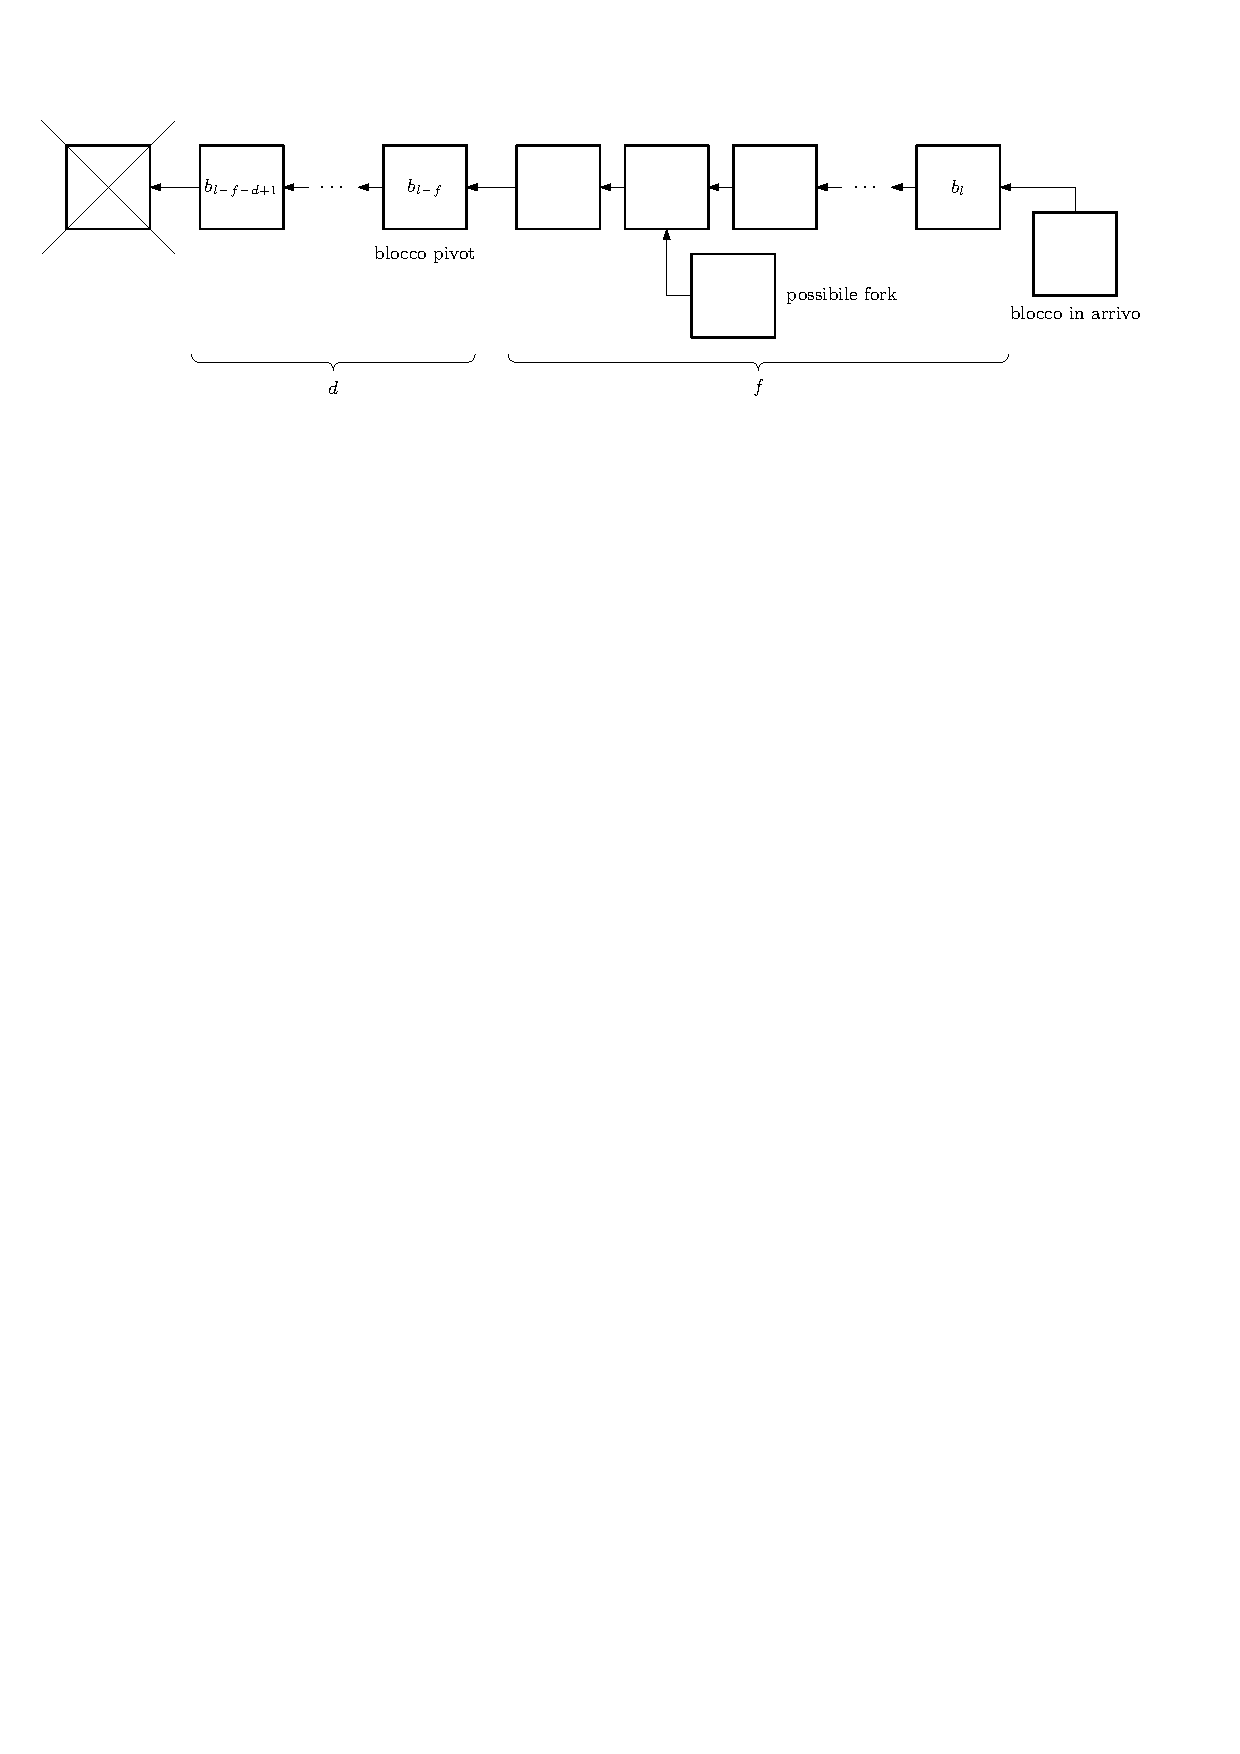
\includegraphics[scale=0.7]{img/capdue/truncated_blockchain.pdf}
	\caption{Blockchain troncata: un nodo memorizza solo gli ultimi $d+f$ blocchi. \emph{Fonte~\cite{bernardini2019blockchains}}}
	\label{fig:blockchain_bern}
\end{figure}

In questo caso si sceglie come blocco pivot $b_{l-f}$, dove $l$ è l'indice dell'ultimo blocco in $\Lambda_N$. Ogni blocco $b_i \in \Lambda_N$ oltre a contenere le transazioni confermate, in una struttura dati autenticata come le altre blockchain (ad esempio Bitcoin), include anche il pADS $\tau_i$, che rappresenta lo stato prima dell'applicazione delle transazioni in $b_i$, che coinvolge solo gli elementi di stato $E_i$ modificati dalle transazioni in $b_i$, il resto è potato, come rappresentato in Figura~\ref{fig:block_content}. Si denota inoltre $\pi_i$ il pADS ottenuto da $\tau_i$ applicando le transazioni in $b_i$: $\pi_i$ non necessita di essere memorizzato e può essere calcolato \emph{al volo} quando è necessario.

\begin{figure}
	\centering
	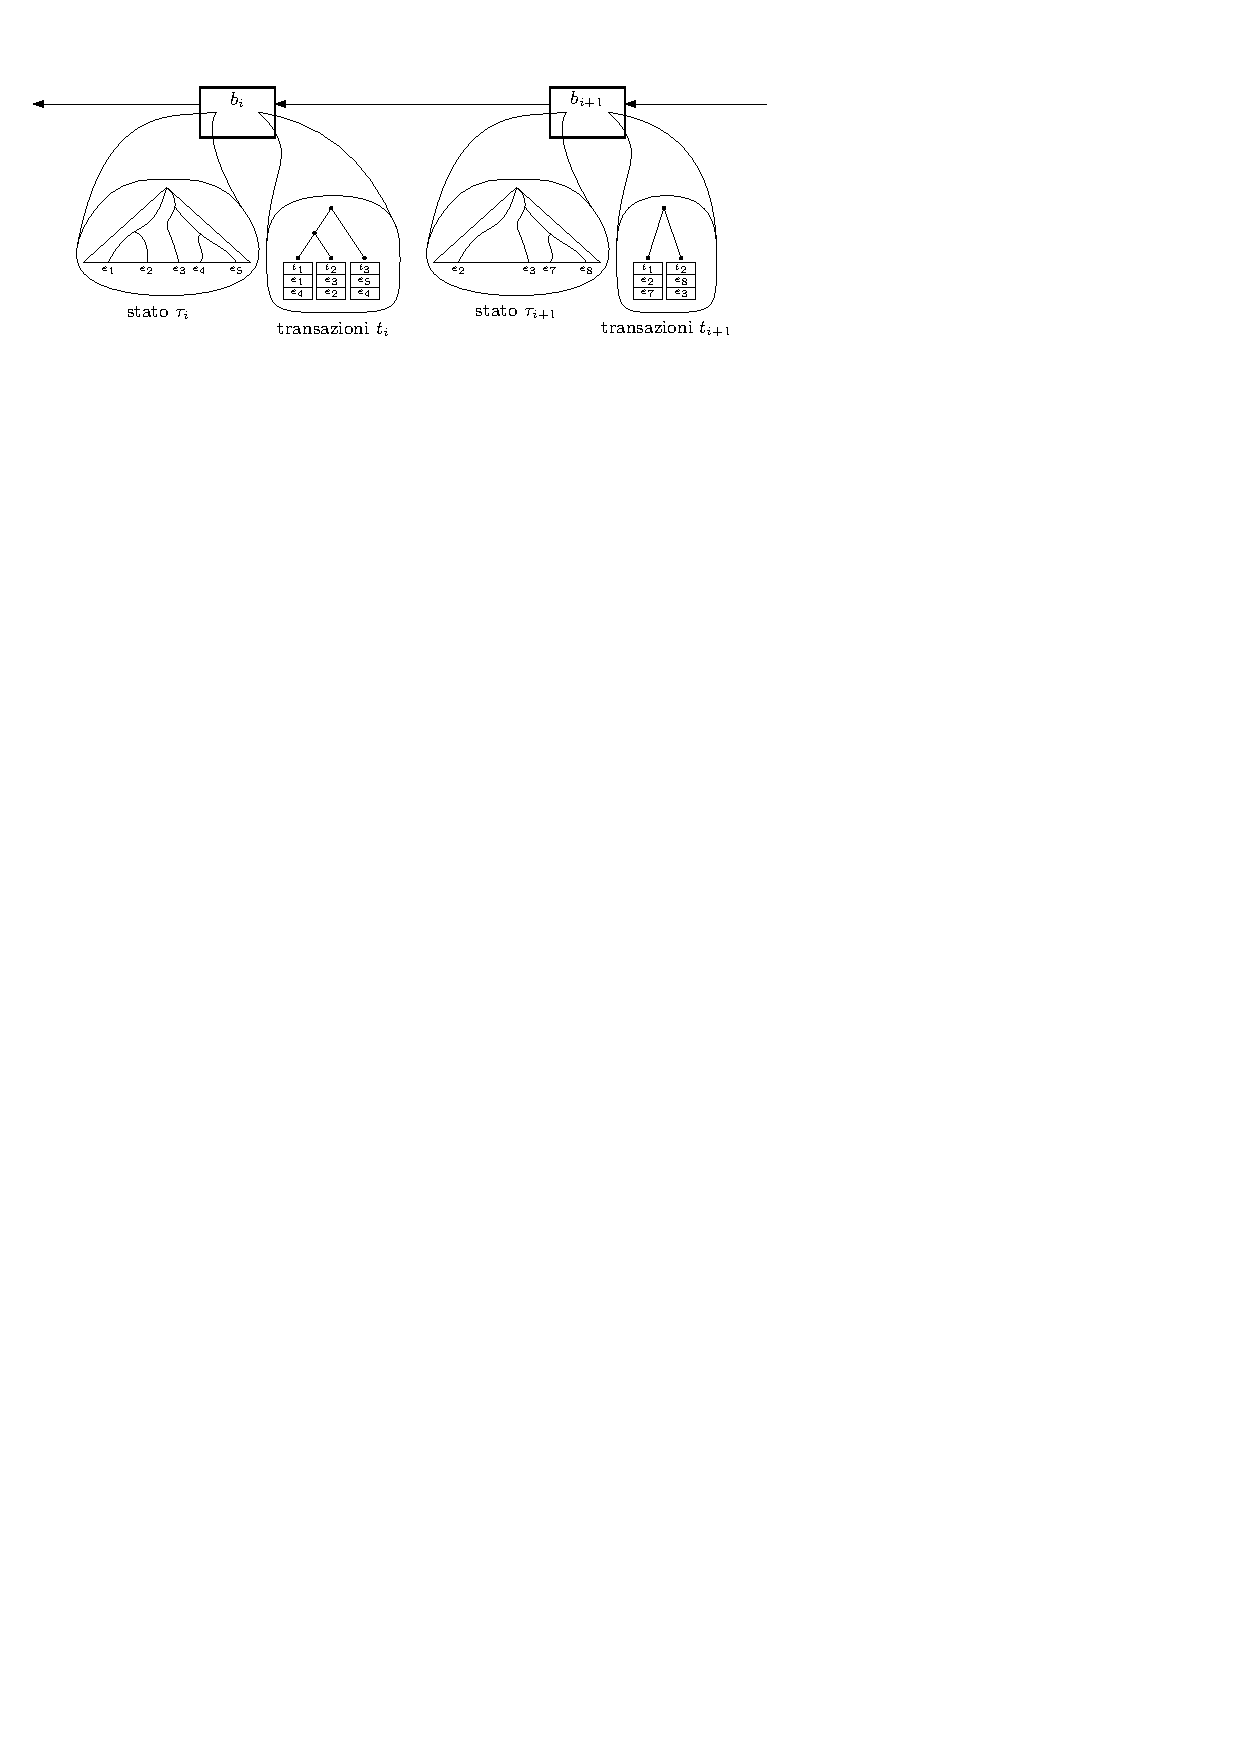
\includegraphics{img/capdue/block_bern.pdf}
	\caption{Contenuto di un blocco. Ognuno blocco $b_i$ contiene le transazioni confermate $t_i$ e il Merkle Tree potato $\tau_i$ contenente solo le foglie degli elementi di stato modificati in $t_i$. \emph{Fonte~\cite{bernardini2019blockchains}}}
	\label{fig:block_content}
\end{figure}

Per la creazione del prossimo blocco $b_{l+1}$ da inserire in blockchain, vengono selezionate tutte le transazioni in attesa dal pool di transazioni. Per ogni elemento di stato $e \in E_{l+1}$, si verifica l'integrità di $\delta_i(e) = \langle v, p, i \rangle$, imponendo $i \geq l-f-d+1$ (in caso contrario la transazione sarebbe troppo vecchia), e comparando il root-hash calcolato da $p$ e da $v$, secondo quanto descritto nel Paragrafo~\ref{sec:ads}, con il root-hash di $\tau_i$ contenuto nel blocco $i$. Se una delle due condizioni non è valida, le transazioni che coinvolgono quell'elemento di stato vengono scartate.
Per il calcolo di $\tau = \tau_{l+1}$, rappresentante lo stato prima dell'applicazione delle transazioni nel futuro blocco $b_{l+1}$ si procede secondo l'Algoritmo~\ref{alg:tau_compute}.
Sia $\delta$ la lista contenente tutte le $\delta_i(e)$ per ogni $e \in E_{l+1}$. Inizialmente si effettua un merge delle proof contenute in $P$, ottenuta estraendole da $\delta$, considerando solo la topologia e non gli hash. Poi si itera partendo da $x = l$ decrementandola fino all'indice del blocco più vecchio, eseguendo per ogni iterazione le seguenti operazioni: (1) si riempiono i nodi di $\tau$ ancora vuoti con $\pi_x$, e (2) la stessa cosa con $\delta_x$, mediante la procedura \emph{fillEmpty}. La procedura si ripete finche $\tau$ non è pieno. La correttezza di \emph{computeState} è data dal fatto che si da precedenza ai nodi più aggiornati nel tempo, mentre gli hash non presenti in $\pi_x$, poiché gli elementi di stato relativi non sono stati modificati nelle transazioni contenute nel blocco $b_x$, sono ottenuti da $\delta_x$.
A questo punto, dopo aver ottenuto lo stato attuale $\tau_{l+1}$ si verifica che ogni transazione $t$ da includere nel blocco rispetta le regole di consenso (ad esempio, non effettua double spending) e la inserisce in $b_{l+1}$. Si esegue l'algoritmo di consenso distribuito e si invia in broadcast il nuovo blocco.
\begin{algorithm}
	\caption{Calcolo di $\tau$}
	\begin{algorithmic}
		\Procedure{computeState}{$\delta$}
			\State{$P \leftarrow$\Call{map}{snd, $\delta$}}
			\State{$\tau \leftarrow$\Call{topologicalMerge}{$P$}}
			\For{$ x \leftarrow l$ \textbf{down to} $l-f-d+1$}
				\State \Call{fillEmpty}{$\tau, \pi_x$}
				\State \Call{fillEmpty}{$\tau, \delta_x$}
				\If{\Call{isFull}{$\tau$}}
					\State{\textbf{break}}
				\EndIf
			\EndFor
			\Return $\tau$
		\EndProcedure
	\end{algorithmic}
	\label{alg:tau_compute}
\end{algorithm}

Alla ricezione del nuovo blocco $b_{l+1}$ un nodo confronta il root-hash ottenuto da $\pi_l$ con il root-hash di $\tau_{l+1}$.  Ogni transazione $t \in b_{l+1}$ viene validata secondo le regole di consenso, utilizzando $\tau_{l+1}$. Se tutte le regole di consenso sono rispettate, $b_{l+1}$ viene inserito, mentre $b_{l-d-f+1}$ viene rimosso da $\Lambda_N$. Il nuovo pivot diventa $b_{l-f+1}$ ed i nodi di storage applicano le transazioni contenute in $b_{l-f+1}$ a $\tau_{l-f+1}$, aggiornando autonomamente le proprie pADS.

\section{Sharding}\label{sec:sharding}

Un'altra proposta in letteratura per risolvere il blockchain scalability trilemma è lo \emph{sharding}, una tecnica impiegata nei database distribuiti, che consiste nel partizionare lo stato della blockchain in molteplici \emph{shard}, gestite in parallelo da differenti sottoinsiemi di nodi, in modo da ridurre l'overhead dei protocolli di consenso e consentire un processamento delle transazioni parallelo tra i vari shard, aumentando il throughput complessivo del sistema e diminuendo il tempo di conferma di una transazione.
Esempi di blockchain che utilizzano questa tecnica sono Elastico~\cite{luu2016secure}, OmniLedger~\cite{kokoris2018omniledger} e RapidChain~\cite{zamani2018rapidchain}.

I protocolli che fanno uso dello sharding in ambito database hanno l'obiettivo di migliorare le performance in ambiente distribuito~\cite{cattell2011scalable, corbett2013spanner}.
Tuttavia essi non possono essere estesi alle blockchain, poiché gli ambiti di impiego sono opposti: mentre nei database, si assume come modello di fallimento quello secondo cui un nodo può non rispondere a richieste o per un problema hardware (come ad esempio, assenza di corrente elettrica, problemi di rete, danneggiamento di hard disk) o per un problema software (ad esempio per un crash del programma), in ambito blockchain l'ambiente di esecuzione è più ostile. Infatti i nodi, oltre che danneggiarsi, possono adoperare comportamenti malevoli.

Gli aspetti fondamentali di una blockchain sharded che ne garantiscono correttezza e sicurezza sono: (1) selezione periodica e randomica dei nodi che compongono una shard con metodologie resilienti ad attacchi di tipo Sybil, e (2) gestione delle transazioni \emph{cross-shard}, in cui gli input ed output riguardano due o più shard.

\paragraph*{Modello di riferimento}
In OmniLedger, la rete è composta da $n$ \emph{validatori}, con il compito di processare le transazioni generate dagli utenti del sistema. Gli $n$ validatori sono uniformemente distribuiti tra $m$ shard, i quali processano solo una parte delle nuove transazioni. Denotato $s_i$ ed $s_j$ le transazioni processate dagli shard $i$ e $j$ rispettivamente, con $i, j \in \{1,\dots,m\}$, e $i \neq j$, $s_i$ ed $s_j$ sono due insiemi disgiunti. Ogni validatore $i$ ha una coppia chiave pubblica $pk_i$ e privata $sk_i$. Il tempo è suddiviso in intervalli di tempo fissi tra i quali avvengono delle riconfigurazioni degli shard, denominati \emph{epoche}. Ogni epoca è composta da un certo numero di \emph{round} nei quali ogni shard processa le transazioni di cui è responsabile. Per partecipare all'epoca $e$, un validatore deve registrarsi entro la fine dell'epoca $e-1$, secondo un procedimento che stabilisca la sua identità resiliente ad attacchi Sybil. Esiste infatti una blockchain che contiene le identità di tutti i validatori registrati. Infine si denota con $f$ il numero di validatori Bizantini, tale che $n = 4f$, ovvero al massimo il $25\%$ dei validatori è malevolo. Il modello di RapidChain è simile, con $f \leq 33\%$.

\paragraph*{Formazione di uno shard}
La formazione degli shard di cui è composta la rete, affinché sia sicura, viene effettuata randomicamente, sulla base di un numero random senza alcun bias e imprevedibile. Mentre alcuni sistemi~\todo{citare sistemi sharded con beacon per generazione numeri random} utilizzano un \emph{beacon} fidato per la generazione di numeri random, altri, come OmniLedger e RapidChain, si basano su un generatore di numeri casuali distribuito. Il primo si basa sulla combinazione del protocollo RandHound~\cite{syta2017scalable} e VRF~\cite{micali1999verifiable}, mentre il secondo si basa su Verifiable Secret Sharing (VSS)~\cite{pedersen1991non}.
RandHound si affida ad un leader per l'orchestrazione del protocollo: se la sua elezione fosse deterministica, un utente malevolo può sfruttare la situazione a proprio vantaggio e portare fino a $fn$ fallimenti. La selezione è quindi randomica, mediante l'uso della VRF. Ogni validatore $i$ genera un valore $t_{i,e,v} =$VRF$_{sk_i}("leader" || config_e || v)$, dove $config_e$  è la lista contenente tutti i validatori registrati per l'epoca $e$ e $v$ è un contatore. Ogni validatore invia il proprio $t_{i,e,v}$, selezionando il minore che riceve e accettando il corrispondente come leader. Se il leader fallisce nell'iniziare la procedura di RandHound, $v$ viene incrementato e riparte la selezione. Il leader genera mediante RandHound ed invia in broadcast a tutti i validatori un numero random $rnd_e$ insieme alla sua prova di correttezza. $rnd_e$ verrà utilizzato da ogni validatore per determinare lo shard a cui è stato assegnato.
Dal punto di vista della sicurezza, un utente malevolo può essere selezionato come leader. Egli può scegliere di cooperare al protocollo, oppure di fallire, venendo escluso per tutta l'epoca $e$. Si noti che non può generare più numeri casuali e proporre quello che più lo soddisfa (ad esempio, un numero tale che porti ad una permutazione in cui tutti i nodi malevoli sono in uno shard), poiché questo dipende da $v$. Infine, la probabilità che un utente onesto sia selezionato dopo che un utente malevolo abbia vinto la lotteria, è molto alta, poiché la probabilità che l'utente malevolo sia selezionato $a$ volte di fila, decresce esponenzialmente con $a$, secondo $(f/n)^a$.
Per diminuire l'impatto di attacchi del tipo \emph{join-leave}, in cui un utente malevolo che entra a far parte di uno shard si disconnette durante l'epoca $e$, viene effettuato uno swap periodico dei nodi tra uno shard e l'altro, spostando solamente $k = \log \frac{n}{m}$ nodi alla volta, per diminuire l'overhead necessario alla risincronizzazione dei nodi che cambiano shard. La risincronizzazione consiste nel download della blockchain dello shard. Per ridurre la dimensione si può attuare un meccanismo di potatura/checkpoint come in~\cite{bernardini2019blockchains, kokoris2018omniledger, leung2019vault}. In RapidChain, un nodo scarica solo l'insieme delle \emph{unspent transaction} (UTXO) di uno shard, sufficienti a verificare le future transazioni.

\paragraph*{Comunicazione cross-shard}
Lo sharding permette di ridurre lo spazio richiesto dalla blockchain, ma allo stesso tempo aumenta la difficoltà della verifica delle transazioni, perché gli input e gli output possono risiedere su shard differenti. Sia $t$ la transazione generata da un utente. $t$ ha un numero $N$ di input $I_1, \dots, I_N$ e un output $O$. Senza perdità di generalità, si può considerare che ad ogni input corrisponda un unico shard.\todo{da rivedere la frase, forse non si capisce bene} Quindi, si denotano gli shard di input ed output con $C_{in}^j$, tale che $j \in \{1, \dots, N\}$, e con $C_{out}$, rispettivamente. 
In OmniLedger, per processare ogni transazione $t$ in modo atomico tra shard, si utilizza un protocollo denominato \emph{Byzantine Shard Atomic Commit}, al cui termine $t$ è o confermata o abortita. Il protocollo è formato da 3 step (vedi Figura~\ref{fig:atomix}):

\begin{figure}
	\centering
	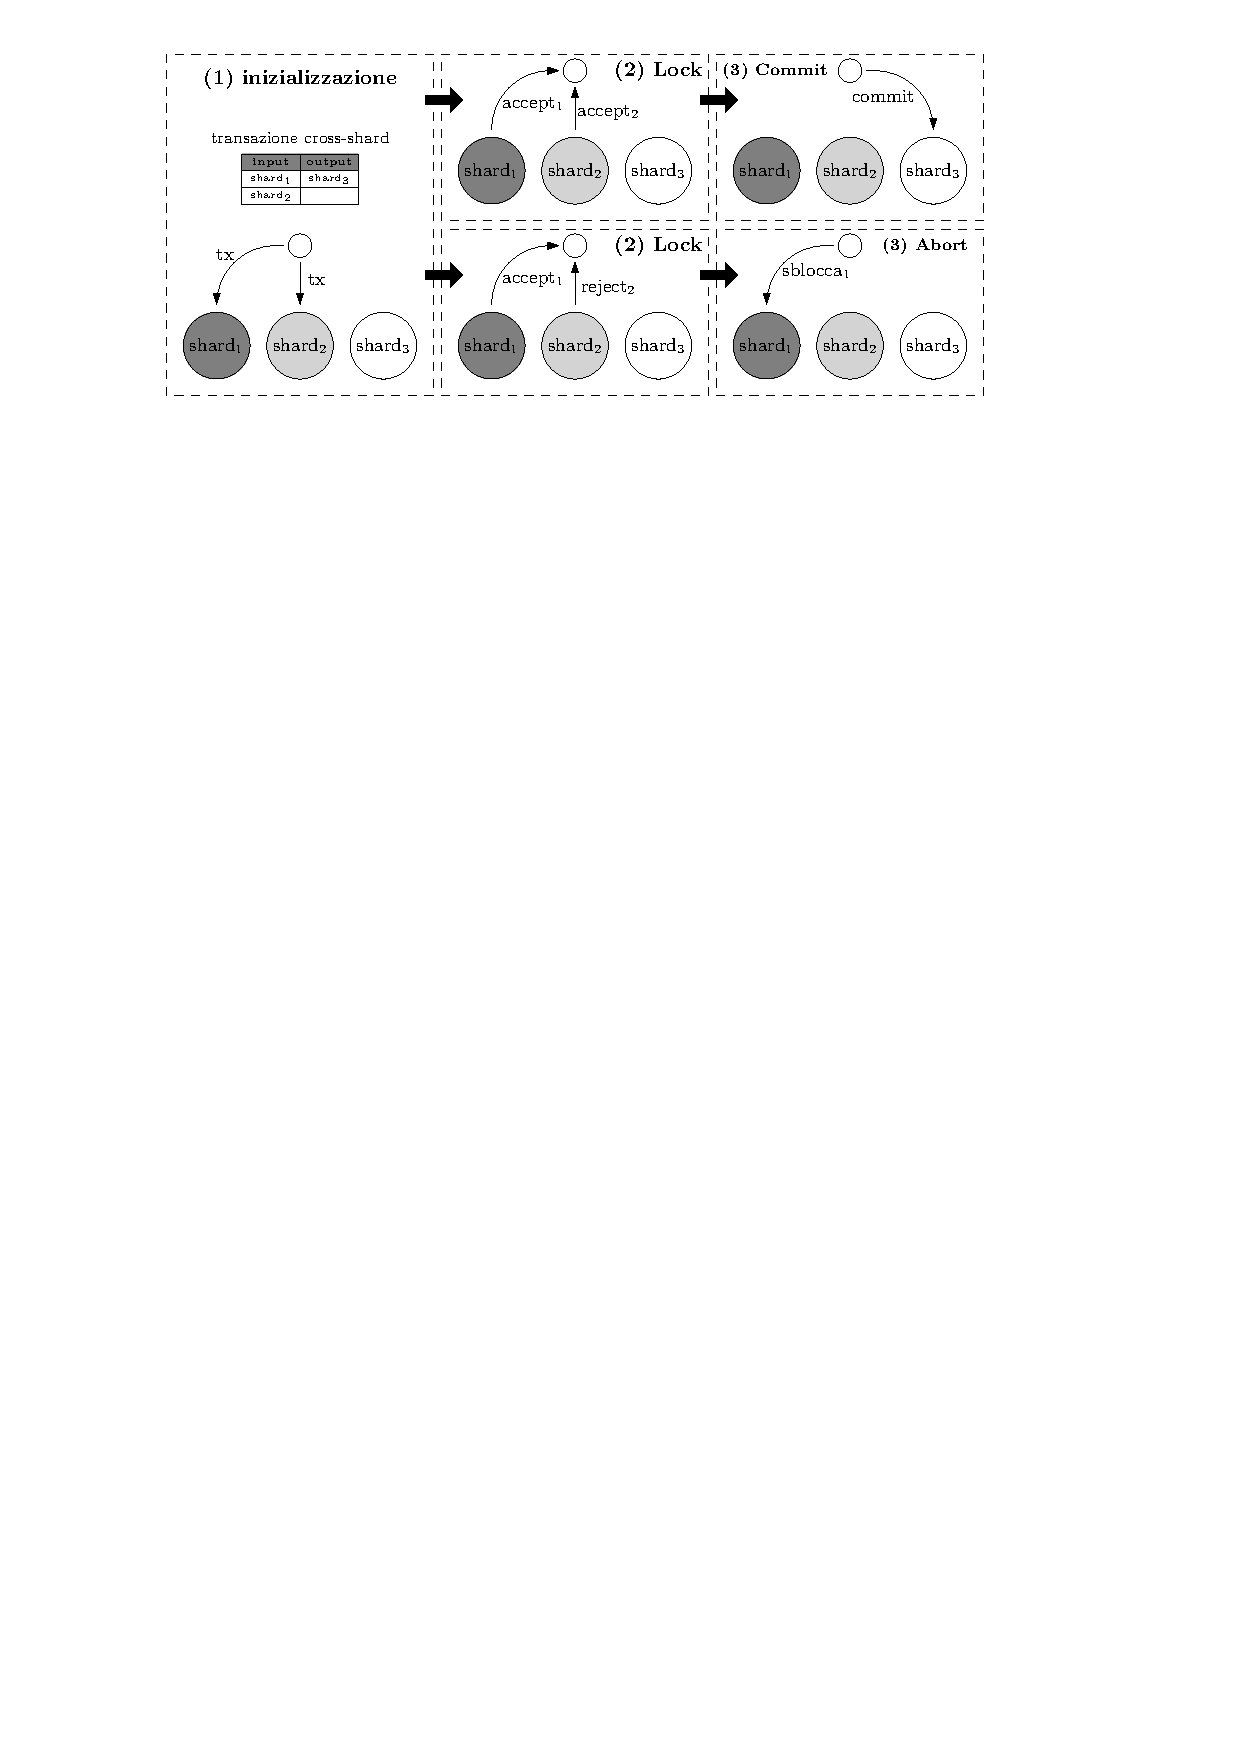
\includegraphics[scale=0.9]{img/capdue/atomix.pdf}
	\caption{Processamento di una transazione cross-shard in Omniledger. \emph{Fonte~\cite{kokoris2018omniledger}}}
	\label{fig:atomix}
\end{figure}

\begin{enumerate}
	\item \textbf{Inizializzazione}: il client $c$ invia $t$ a tutte i $C_{in}^j$ per ogni input $j$ $I_j$ in $t$.
	\item \textbf{Lock}: Ogni leader di $C_{in}^i$ verifica la validità della transazione, ovvero se l'input di cui è responsabile $C_{in}^i$ è spendibile. Se la transazione è valida, il leader imposta la UTXO associata come spesa (quindi bloccata), ed invia a $c$ una \emph{proof-of-acceptance}, ovvero una proof di un Merkle Tree del blocco in cui la transazione è stata inserita. Se non è valida, $c$ riceve una \emph{proof-of-rejection}.
	\item \textbf{Unlock}: in base alla precedente fase il client può confermare o abortire la transazione:
	
	\begin{enumerate}
		\item \textbf{Unlock to commit}: se tutti i $C_{in}^i$ rispondono con una \emph{proof-of-acceptance}, $c$ può confermare la transazione. Crea quindi una transazione \emph{unlock-to-commit} destinata a $C_{out}$ contenente tutte le \emph{proof-of-accemptance} per ogni input e $C_{out}$ crea una nuova UTXO destinata all'output di $t$;
		\item \textbf{Unlock to abort}: se riceve almeno una \emph{proof-of-rejection}, $c$ può richiedere di sbloccare le UTXO per gli input $I_j'$ per i quali ha ricevuto una \emph{proof-of-acceptance}. $c$ crea quindi una transazione \emph{unlock-to-abort} dove inserisce almeno una \emph{proof-of-rejection} per un input in modo tale da sbloccare la UTXO associata.
	\end{enumerate}

\end{enumerate}

Questa soluzione non richiede una comunicazione inter-sharding, ma genera un grande overhead di comunicazione dovuta ad ogni proof generata per ogni input della transazione $t$. Inoltre, un altro aspetto negativo è che richiede del lavoro aggiuntivo, rispetto alla semplice e sola creazione di una transazione, al client, rendendolo più difficile da utilizzare per dispositivi semplici, come quelli IoT.

RapidChain risolve questo problema nel modo seguente. L'utente che crea $t$, invia $t$ a $C_{out}$\footnote{secondo un meccanismo di \emph{inter-committee routing} molto efficiente basato sull'algoritmo di routing di Kademlia~\cite{maymounkov2002kademlia}}. Il leader di $C_{out}$ per ogni input $I_j$ di $t$, genera una transazione $t_i$ con input $I_j$ ed output $I_j'$, con $|I_j| = |I_j'|$ (con lo stesso valore) e $I_j'$ è diretta sul conto di $C_{out}$. Infine genera la transazione $t_{N+1}$, avente input $I_j'$, con $j \in \{1, \dots, N\}$ e output $O$. Il leader invia $t_i$ ad ogni $C_{in}^i$ e se $t_i$ è confermata, $C_{in}^i$ invia $I_i'$ a $C_{out}$. Se tutte le transazioni $t_i$, con $i \in \{1, \dots, N\}$ sono confermate, allora $C_{out}$ inserisce $t_{N+1}$ nella propria blockchain.


\paragraph*{}
Sebbene lo sharding possa rappresentare una soluzione alla scalabilità, in modo da migliorare l'utilizzo dell'hash power complessivo della rete e ridurre l'overhead di storage per la memorizzazione dell'intero stato della blockchain, la sicurezza può essere un problema: è più facile per un attaccante prendere il controllo di una singola shard, a causa del ridotto numero di partecipanti presenti nello shard stesso, secondo l'attacco noto in letteratura come \emph{1\% attack}, o \emph{single-shard  takeover attack}~\cite{chauhan2018blockchain}. Secondo questo attacco, per una rete composta da $m=100$ shard, ad un attaccante è necessario solo l'1\% dell'hash power totale per attuare i suoi comportamenti malevoli, come quelli descritti nel Paragrafo~\ref{attacks}.